\documentclass[a4paper]{article}

\usepackage[english]{babel}
\usepackage[utf8x]{inputenc}
\usepackage{graphicx}
\usepackage{amsthm}
\usepackage{amssymb}
\usepackage{amsmath}
\usepackage{nicematrix}
\usepackage{tensor}
\usepackage{physics}
\usepackage{xcolor}
\usepackage{enumitem}
\usepackage{pgfplots}
\usepackage{booktabs}
\usepgfplotslibrary{fillbetween}

\usepackage[backend=biber,style=ieee,citestyle=numeric-comp,sorting=none]{biblatex}
\addbibresource{sample.bib}

\newtheorem{remark}{Remark}[section]
\newtheorem{definition}{Definition}[section]
\theoremstyle{definition}
\newtheorem{lemma}{Lemma}[section]
\newtheorem{theorem}{Theorem}[section]
\newtheorem{example}{Example}[section]
\newtheorem{corollary}{Corollary}[section]
\newtheorem{condition}{Assumption}[section]
\newtheorem{insight}{Insight}[section]
\newtheorem{problem}{Problem}[section]
\newtheorem*{solution}{Solution}

\title{Math Prep Course Day One}
\author{Ashhad}

\begin{document}

\maketitle

\section{Exercises in BK-V3}
There was really one this one problem I found interesting whose solution wasn't available in the document, so I decided to include it. The rest are either MCQ-type questions or exercises that have a sufficient enough sketch that a complete solution isn't necessary.

\begin{problem}
Specify a spiral in parametric representation.
\end{problem}
\begin{solution}
This problem is best accomplished with simply playing around with polar functions on some graphing tool, but intuitively a spiral looks something like this

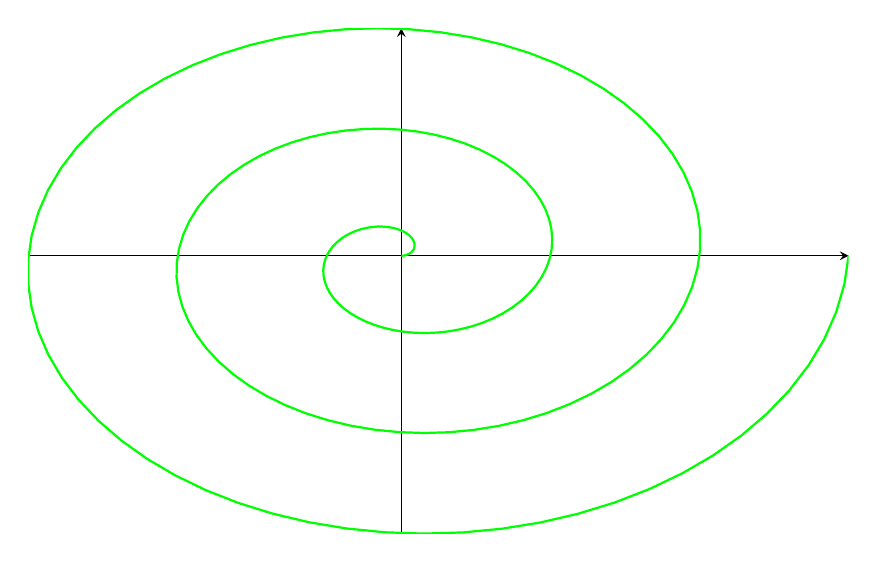
\begin{tikzpicture}
\begin{axis}[axis lines=middle, 
    width = 12cm, height =8cm,
    ticks=none]

\addplot[color=green, samples=200, domain=0:6*pi, thick]
  ({x*cos(deg(x))}, {x*sin(deg(x))});

\end{axis}
\end{tikzpicture}

Our objective now is to find such a formula that traces this graph. In polar coordinates, the following function suffices
\[
r = \theta
\]

Converting this over to pure cartesian coordinates we obtain
\begin{align*}
r &= \theta \\
\sqrt{x^2 +y^2} &= \arctan(\frac{y}{x})
\end{align*}
\end{solution}

But this solution is generally not very nice, instead a better solution can be obtained if we instead solve for parameterization via theta
\begin{align*}
x = r\cos(\theta) && y = r\sin(\theta) \\
x = \theta\cos(\theta) && y = \theta\sin(\theta) && \because r = \theta
\end{align*}

\section{Quadratic Equations}

\begin{problem}
Find the roots
\[
x^2 - 4x + 3 = 0
\]
\end{problem}
\begin{solution}
We may solve by factorization as follows
\begin{align*}
x^2 -4x +3  &= x^2 -x -3x +3 \\
    &=x(x-1) - 3(x-1) \\
    &= (x-3)(x-1) \\
x-3 = 0 &\implies x=3 \\
x-1 = 0 &\implies x=1
\end{align*}

\begin{tikzpicture}
\begin{axis}[axis lines=middle,
    ymin=-1.5,
    width = 12cm, height =8cm,]

\addplot[color=blue, thick, domain=0:5]{x^2 -4*x + 3};
\end{axis}
\end{tikzpicture}
\end{solution}


\begin{problem}
Find the roots
\[
x^2 + x + 1 = 0
\]
\end{problem}
\begin{solution}
Since this equation is not straightforward to factorize, we solve using the quadratic formula
\begin{align*}
\frac{-b \pm \sqrt{b^2 - 4ac}}{2a} &= \frac{-1 \pm \sqrt{1^2 - 4(1)(1)}}{2(1)} \\
    &= \frac{-1 \pm \sqrt{-3}}{2}
\end{align*}
Since the roots are complex, plotting there isn't a graph that we can sketch that encodes the solutions
\end{solution}


\begin{problem}
Find the roots
\[
x^2 - 3x + 1 = 0
\]
\end{problem}
\begin{solution}
Again, this problem is not easily factorize, thus we rely on the quadratic formula once more
\begin{align*}
\frac{-b \pm \sqrt{b^2 - 4ac}}{2a} &= \frac{3 \pm \sqrt{3^2 - 4(1)(1)}}{2(1)} \\
    &= \frac{3 \pm \sqrt{5}}{2}
\end{align*}
\begin{tikzpicture}
\begin{axis}[axis lines=middle,
    ymin=-1.5,
    width = 12cm, height =8cm,]

\addplot[color=blue, thick, domain=-1:4]{x^2 -3*x + 1};
    \pgfmathsetmacro{\rA}{(3 - sqrt(5))/2}
    \pgfmathsetmacro{\rB}{(3 + sqrt(5))/2}

    % Add markers at (root,0)
    \addplot[only marks,mark=*] coordinates {(\rA,0) (\rB,0)};
    
    % Add labels near them
    \node[above right] at (axis cs:\rA,0) {$\tfrac{3 - \sqrt{5}}{2}$};
    \node[above left] at (axis cs:\rB,0) {$\tfrac{3 + \sqrt{5}}{2}$};
\end{axis}
\end{tikzpicture}
\end{solution}

\section{Functions and Mapping}

\begin{problem} Is the following a function?
\[
f(x) = x^3
\]
\end{problem}
In all of these solutions, we must show uniqueness, that means that if we draw any vertical line it cannot intersect more than one point on the curve. \\
\begin{tikzpicture}
\begin{axis}[axis lines=middle,
    width = 12cm, height =8cm,
    scaled ticks = false]
\addplot[color=blue, thick, domain=-100:100]{x^3};
\end{axis}
\end{tikzpicture}

\begin{solution}
Here, we can see that no vertical line intersects the curve more than once (At higher values the curve becomes very steep- so it may look like its not unique, but if you zoom in it still is!)
\end{solution}

\begin{problem}
Is the following a function?
\[
f(x) = x^2
\]
\end{problem} 

\begin{tikzpicture}
\begin{axis}[axis lines=middle,
    width = 12cm, height =8cm,
    scaled ticks = false]

\addplot[color=red, thick, domain=-100:100]{x^2};
\end{axis}
\end{tikzpicture}

\begin{solution}
Here it is also easy to see that no vertical line passes through two points of the curve..
\end{solution}


\begin{problem}
Is the following a function?
\[
f(x,y) = x^2 + y^2 - 1
\]
\end{problem}

\begin{center}
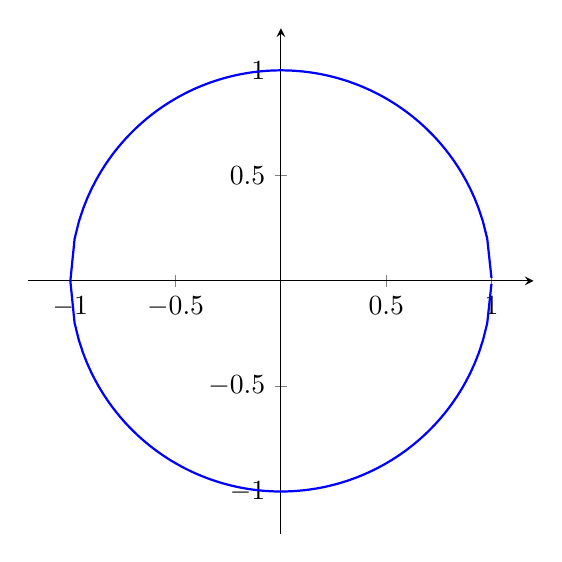
\begin{tikzpicture}
\begin{axis}[axis lines=middle,
    ymin=-1.2, ymax=1.2, xmin=-1.2, xmax=1.2,
    width = 8cm, height =8cm]

\addplot[color=blue, thick, samples = 100, domain=-1:1]{sqrt(1-x^2)};
\addplot[color=blue, thick, samples = 100, domain=-1:1]{-sqrt(1-x^2)};
\end{axis}
\end{tikzpicture}
\end{center}

\begin{solution}
Now here, any vertical line between \((-1, 1)\) intersects the circle at two points. Therefore this curve does not correspond to a unique function
\end{solution}

\begin{problem}
Is the following a function?
\[
f(x,y) = x^2 - y^2 - 1
\]
\end{problem}

\begin{center}
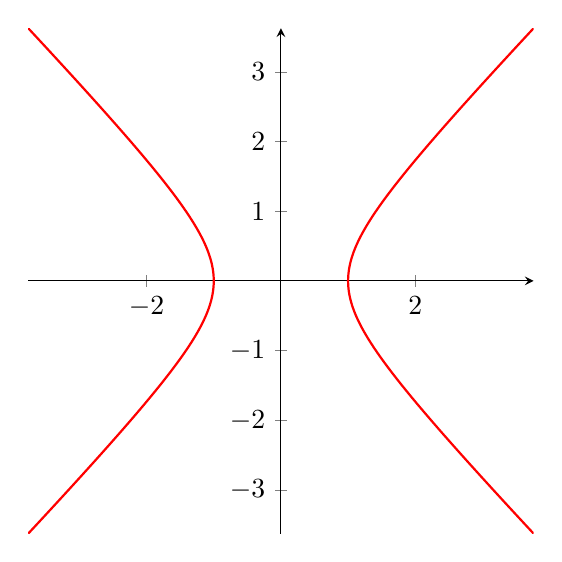
\begin{tikzpicture}
\begin{axis}[axis lines=middle,
    width = 8cm, height =8cm]

\addplot[red, thick, domain=-2:2, samples=200]
  ({cosh(x)}, {sinh(x)});
\addplot[red, thick, domain=-2:2, samples=200]
  ({-cosh(x)}, {sinh(x)});
\end{axis}
\end{tikzpicture}
\end{center}

\begin{solution}
Any horizontal line drawn in the region \((-\infty, -1) \cup (1, \infty)\) intersects the hyperbola at two points, therefore this function isn't unique either.
\end{solution}


\begin{problem}
Find the range (I think?)
\begin{align*}
f(x) = \frac{3}{x} -1 && x \in (\frac{1}{3}, 1) \cup (3, \infty)
\end{align*}
\end{problem}
\begin{solution}
First we note that our function is continuous on both of the domains we are given (Since it is only undefined at zero, it blows up to infinity there), therefore it will be sufficient to simply evaluate the function on the endpoints of the domain to obtain the range intervals
\begin{align*}
f(1/3) &=\frac{3}{\frac{1}{3}} - 1 = 9-1 = 8 \\
f(1) &= \frac{3}{1} -1 = 2 \\
f(3) &= \frac{3}{3} -1 = 0 \\
f(x)_{Lim\ x \to \infty} &= Lim_{x\to \infty} \frac{3}{x} - 1 = 0 - 1 = -1
\end{align*}
Our range is therefore
\[
(2, 8) \cup (-1, 0)
\]
\end{solution}

\begin{problem}
\begin{align*}
f(x) = 3x-1, \ g(x) =\frac{x}{3} - \frac{1}{3}
\end{align*}
Find \(g(f(x))\)
\end{problem}
\begin{solution}
\begin{align*}
g(f(x)) &= \frac{f(x)}{3} - \frac{1}{3} \\
    &= \frac{3x - 1}{3} - \frac{1}{3} \\
    &= \frac{3x}{3} - \frac{1}{3} -\frac{1}{3} \\
    &= x -\frac{2}{3}
\end{align*}
\end{solution}

\begin{problem}
Given the function
\begin{align*}
f(x) = x^2
\end{align*}

\begin{tikzpicture}
\begin{axis}[axis lines=middle,
    width = 12cm, height =8cm,
    scaled ticks = false]

\addplot[color=blue, thick]{x^2};
\end{axis}
\end{tikzpicture}

Find the following transformations: \\ \(x \to x+2\)\\ \(f(x) \to f(x)-4\)\\ \(x \to x-2, f(x) \to 2f(x)\).
\end{problem}
\begin{solution}
This is more of a graphic problem than algebraic, one thing to keep in mind is that transformation to ranges are (in general) always preceded by transformation in domains. For the first problem, we have
\begin{align*}
f(x') &= f(x+2) \\
    &=(x+2)^2
\end{align*}

\begin{tikzpicture}
\begin{axis}[axis lines=middle,
    width = 12cm, height =8cm,
    scaled ticks = false]

\addplot[color=red, thick, domain=-5:1]{(x+2)^2};
\end{axis}
\end{tikzpicture}

For the second, we may write
\begin{align*}
f'(x) &= f(x) - 4 \\
    &= x^2 -4
\end{align*}

\begin{tikzpicture}
\begin{axis}[axis lines=middle,
    ymax=12,
    width = 12cm, height =8cm,
    scaled ticks = false]

\addplot[color=green, thick]{x^2 -4};
\end{axis}
\end{tikzpicture}

And for the third 
\begin{align*}
f'(x') &= f'(x-2) \\
    &= 2f(x-2) \\
    &= 2(x-2)^2
\end{align*}
\end{solution}

\begin{tikzpicture}
\begin{axis}[axis lines=middle,
    width = 12cm, height =8cm,
    scaled ticks = false]

\addplot[color=blue, thick, domain=-2:6]{2*(x-2)^2};
\end{axis}
\end{tikzpicture}

\begin{problem}
\begin{align*}
f(x) = 3x^2 + 2, \ g(x) = \sqrt{3 - \frac{x}{2}}
\end{align*}
Find the Domain of \((f+g)(x)\) and Range of \((g(f(x))\)
\end{problem}
\begin{solution}
The domain of \(f(x)\) is the entirety of \(\mathbb{R}\). So, we only need to focus on the domain of \(g(x)\). Since a square root cannot have a negative value, we look for when the expression inside the square root is negative.
\begin{align*}
3 - \frac{x}{2} &< 0 \\
3 &< \frac{x}{2} \\
6 &< x \implies x > 6
\end{align*}
Thus our domain for \(g(x)\) is \((-\infty, 6]\). Now whenever two functions are composed via addition, the resulting domain is the intersection of the domains of the added functions. \\

Therefore the domain of \((f+g)(x)\) is also \((-\infty, 6]\). \\

For the range, we see that \(f(x)\) ranges \([2, \infty)\), however, this is outside the domain of \(g(x)\)! Therefore, in order to obtain the range of \(g(f(x))\), we first restrict the range of \(f(x)\) to \([2, 6]\) only. Since \(g(x)\) is continuous on this interval, the range is obtained by evaluating \(g\) on the endpoints.
\begin{align*}
g(2) = \sqrt{3 - \frac{2}{2}} = \sqrt{2} \\
g(6) = \sqrt{3 - \frac{6}{2}} = \sqrt{0} = 0 \\
\end{align*}

Therefore our range is \([0, \sqrt{2}]\)
\end{solution}

\begin{problem}
Find the inverse
\begin{align*}
f(x) = \frac{3-x^2}{4}
\end{align*}
\end{problem}
\begin{solution}
\begin{align*}
y &= \frac{3-x^2}{4} \\
4y &= 3 -x^2 \\
4y -3 &= x^2 \\
x &= \sqrt{4y-3}
\end{align*}
The inverse function is therefore \(f^{-1}(y) = \sqrt{4y-3}\)
\end{solution}

\section{LoL}
\begin{problem}
Find the inverse
\begin{align*}
f(x) = \frac{3x^6 - x^5}{x^4 -x^3} + \frac{x^2}{x^{100}}
\end{align*}
Evaluate \(f(f^{-1}(x))\)
\end{problem}
\begin{solution}
I'll maybe try solving this explicitly if I'm unemployed enough.
\begin{align*}
&\frac{3x^5(x-1)}{x^3(x-1)} + \frac{1}{x^{98}} = y \\
&\frac{3x^{100} + 1}{x^{98}} = y \\
&3x^{100} + 1 = yx^{98} \\
&yx^{98} -3x^{100} = 1 \\
&y -3x^2 = \frac{1}{x^{98}} \\
&y = 3x^2 -\frac{1}{x^{98}}
\end{align*}

For now whoever so wishes can attempt to explicitly verify this inverse.
\end{solution}

\end{document}
